\documentclass[a4paper,10pt]{article}
\usepackage[margin=2cm]{geometry}
\usepackage[utf8]{inputenc}



\newcommand{\trnsp}{\mathsf{T}}
\usepackage[round]{natbib}
\renewcommand{\bibname}{References}
\bibliographystyle{abbrvnat}

\usepackage{amsmath, amsfonts}
\usepackage{graphicx}
\usepackage{subfig}
\usepackage{float}
\usepackage{hyperref}
\usepackage{listings}
\usepackage{xcolor}
\hypersetup{colorlinks=true, urlcolor=blue, citecolor=magenta}

\definecolor{codegreen}{rgb}{0,0.6,0}
\definecolor{codegray}{rgb}{0.5,0.5,0.5}
\definecolor{codepurple}{rgb}{0.58,0,0.82}
\definecolor{backcolour}{rgb}{0.95,0.95,0.92}
\lstdefinestyle{mystyle}{
    backgroundcolor=\color{backcolour},
    commentstyle=\color{codegreen},
    keywordstyle=\color{magenta},
    numberstyle=\tiny\color{codegray},
    stringstyle=\color{codepurple},
    basicstyle=\ttfamily\footnotesize,
    breakatwhitespace=false,
    breaklines=true,
    captionpos=b,
    keepspaces=true,
    numbers=left,
    numbersep=5pt,
    showspaces=false,
    showstringspaces=false,
    showtabs=false,
    tabsize=2
}

\lstset{style=mystyle}


\newcommand{\R}{\mathbb{R}}
\newcommand{\N}{\mathcal{N}}


\makeatletter
\@addtoreset{exercise}{section}
\makeatother
\newcounter{exercise}
\newtheorem{exercise}{Exercise}
\renewcommand{\theexercise}{\arabic{exercise}}
\newsavebox{\mybox}
\newenvironment{note}
{
\begin{center}
\begin{lrbox}{\mybox}
\begin{minipage}{42em}}
{\end{minipage}
\end{lrbox}\fbox{\usebox{\mybox}}
\end{center}}
\date{}


\title{Seminars on Overparametrized Machine Learning: \\Hand-in assignment 3}
\author{Antônio H. Ribeiro, Dave Zachariah, Per Mattsson}

\begin{document}

\maketitle
\begin{center}
	\large \textbf{Due: 2nd of December 2021, 23:59}
\end{center}

\textit{
The items in the assignment can be implemented in the programming language of choice.
Nonetheless, we recommend the usage of Python as a programming language, since we might include suggestions of functions and code snippets in the exercise description.}

The setup of this problem resembles that from Figure 2 in~\citep{jacot_neural_2018}.  We try to recover the function $f(x_i) = x_{i1} x_{i2}$ where $x_i = (x_{i1}, x_{i2})$ is a given input.

\paragraph{Dataset:} We consider a dataset consisting only of $n_o = 5$ points $(x_i, y_i)$, $i = 1, 2, 3, 4, 5$. The inputs are two dimensional $x_i \in \R^2$ and the output are computed using the function $f$ is defined as $y_i = f(x_i) = x_{i1} x_{i2}$. All the inputs used for training lie on the unitary circle, and have the format
\begin{equation}
    x_i = (\cos(\gamma_i), \sin(\gamma_i)).
\end{equation}
Where $[\gamma_1, \gamma_2, \gamma_3, \gamma_4, \gamma_5] = [-2, -1.2, -0.4, 0.5, 1.5]$. In Figure 1, we illustrate where the points $x_i$ lie in the plane $\R^2$ and in the one dimensional plot, as a function of the angle $\gamma_i$.



\begin{figure}[H]
    \centering
    \subfloat[Inputs, $x$]{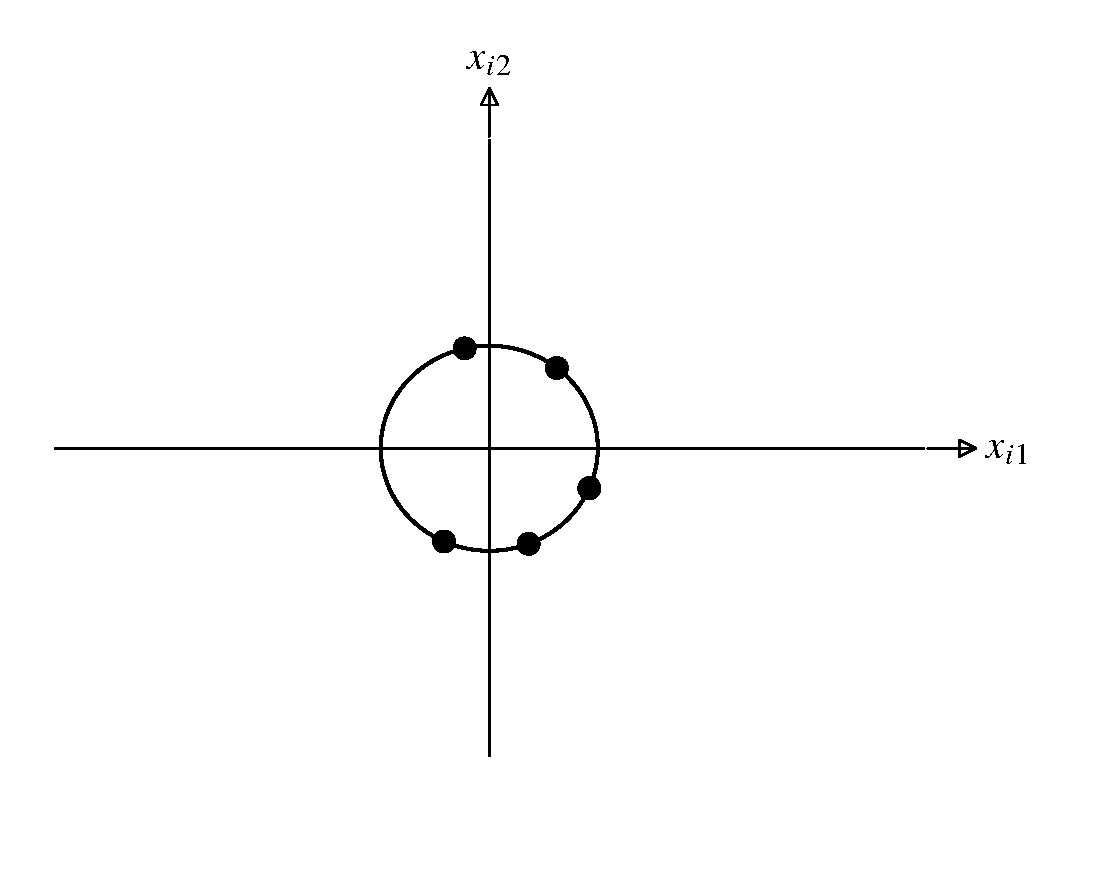
\includegraphics[width=0.43\textwidth]{img/function2d.pdf}}
    \subfloat[Function $f$]{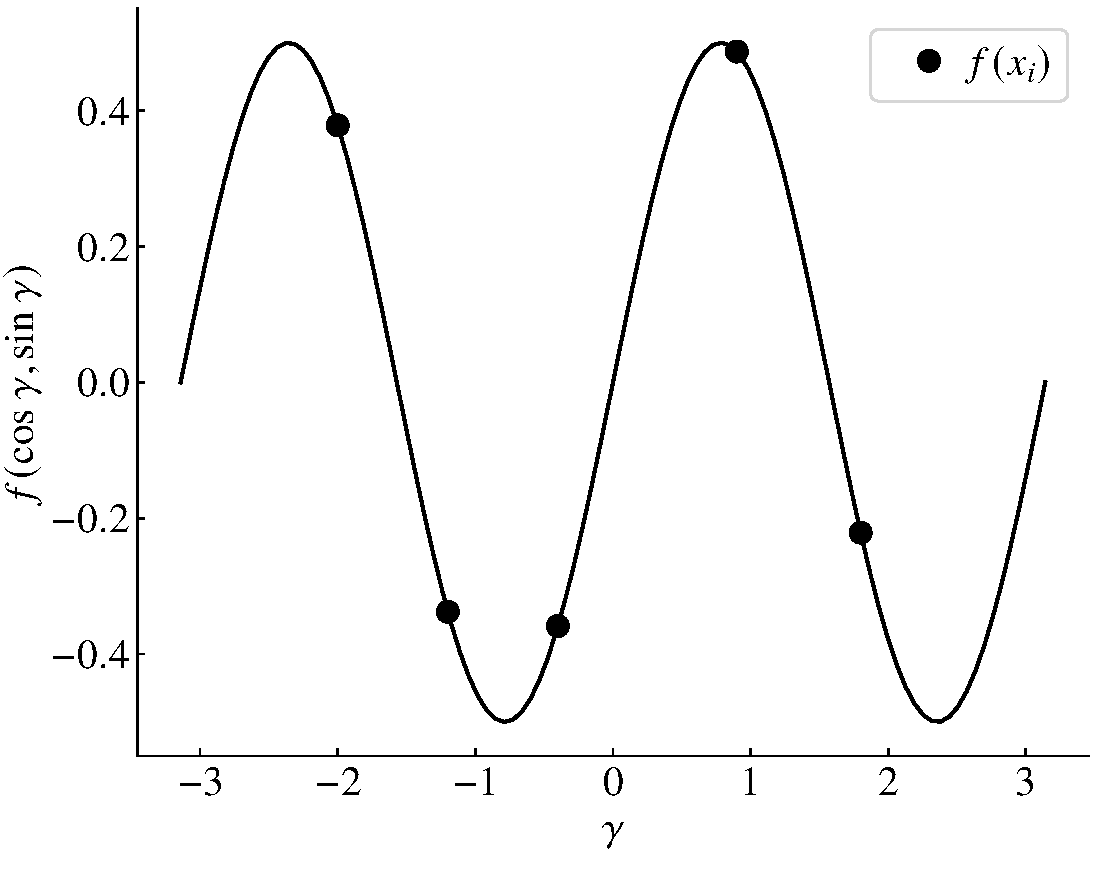
\includegraphics[width=0.43\textwidth]{img/function1d.pdf}}
    \caption{In a), we show the inputs two dimentional inputs $x_i$, $i = 1, \cdots, 5$ together with the unitary circle. In b). we show the function $f(x)$ as we vary the angle $\gamma$, the points $(x_i, f(x_i))$ that will be used for training are indicated by disks.}
    \label{fig:dataset}
\end{figure}

\paragraph{Notation:}  We consider the following notation
\begin{itemize}
    \item \textbf{Obseved points}: We consider $n_o=5$ points were observed and will be used to train the model. We denote the stacked $X_o$ the matrix containing in its rows the observed inputs $x_i$, $i = 1, \cdots, 5$ and $y_o$ the vector containing the corresponding outputs. In general, the sub-index $_o$ will be used to denote quantities obtained from these points.
    \item \textbf{Evaluation points}: We consider $n_e = 100$ evaluation points, obtained for $\gamma$ uniformly spaced in the interval $[-\pi, \pi]$. These points are close together and will be used to generate plots that look like they are a continuous evaluation of the fuction (i.e., they were used to generate the full line in Figure~\ref{fig:dataset}(b)). Here, we denote by $X_e$ the matrix containing in its rows the observed evaluation inputs  and by  $y_e$ the vector containing the corresponding outputs. In general, the sub-index $_e$ will be used to denote quantities obtained from these points.
\end{itemize}

\paragraph{Model:} As a model, we will consider a neural network with $L=4$ hidden layers. The neural network will be a function
$f_{\theta}: \R^2 \rightarrow \R$. Let $\alpha^{(\ell)}\in \R^{n_\ell}$ denote the activations of the neurons at $\ell$-th layer. Defining,  $\alpha^{(0)} = x$, and, recursively,
\begin{equation}
    \label{eq:nn}
    \alpha^{(\ell+1)}(x) = \sigma\left(\frac{1}{\sqrt{n_\ell}} W^{(\ell)} \alpha^{(\ell)}(x)  + \beta b^{(\ell)} \right), \text{ for } \ell = 0, 1, \cdots, L-1,
\end{equation}
the neural network output is an affine transformation of the activations in the last layer $f_{\theta}(x) = W \alpha^{(L-1)}(x) + b$, where we use $W = W^{(L)}$ and $b = b^{(L)}$ to denote the weights and bias in the last layer. The weights $W^{(\ell)}$ and bias of  $b^{(\ell)}_{i}$ have dimension $n_{\ell+1} \times n_{\ell}$ and $n_{\ell+1}$, respectively. At initialization, we consider it entries are are $W^{(\ell)}_{ij} \sim \N(0, 1)$ and $b^{(\ell)}_{i} \sim \N(0, 1)$. As in the original, paper $\beta = 0.1$
and the nonlinearity $\sigma(\cdot)$ is the ReLU activation function, i.e. $\sigma(z) = \max(z, 0)$ applied elementwise.

For simplicity, in this exercise, we consider all hidden layers have the width 1000. Hence, $n_0 =2$ and $n_\ell = 1000$ for $\ell= 1, \cdots, L-1$.



\section*{Part 1: Neural Network as a Gaussian Process}

Neural networks at the initialization tend to Gaussian Processes (GP) in the infinite width limit. This is stated in Proposition 1 from~\citep{jacot_neural_2018} and will be numerically verified here.

\paragraph{Neural network with untrained hidden layers:} Here we consider a neural network where only the last layer is trained. The weights and bias are fixed at initialization values $W^{(\ell)}_{ij} \sim \N(0, 1)$ and $b^{(\ell)}_{i} \sim \N(0, 1)$. And the only parameter that is trained is the parameter vector at the last layer $\theta = \begin{bmatrix}
    W & b
\end{bmatrix}^\trnsp$.  Let by $A_o\in \R^{5 x (1000+1)}$ the matrix containing in its rows the activations in the last layer plus a last colum containin ones. It does it for the 5 observed points,
\begin{equation}
    A_o =
    \begin{bmatrix}
     \alpha^{(L-1)}(x_1) & 1 \\
     \vdots \\
     \alpha^{(L-1)}(x_5) & 1
    \end{bmatrix},
\end{equation}
we can estimate the parameter $\theta$ by a simple linear regression problem, similar to the previous assignments:
\begin{equation}
\label{eq:ls-sol}
\theta = (A_o^\trnsp A_o)^{+} A_o^\trnsp y_o,
\end{equation}
Which, in the overparametrized regime, corresponds to finding the minimum $\ell_2$-norm solution to the problem that minimizes the sum of square error predictions (as used in the previous assignments).

\begin{note}
\textbf{Note:} \href{https://docs.scipy.org/doc/scipy/reference/generated/scipy.linalg.lstsq.html}{scipy.linalg.lstsq} does yield the desired behaviour.
\end{note}

\paragraph{Gaussian Process (GP)} Given a kernel $k: \R^2 \times \R^2 \rightarrow \R$ that maps a pair of inputs $x_i$ and $x_j$ to a real value, i.e. $k(x_i, x_j) \mapsto K_{i, j}$. A Gaussian Process is defined by saying that, when applied to a inputs $\{x_i\}_{i = 1}^n$, the output denoted here by $h(x)$ is jointly normal, that is
\begin{equation}
    \begin{bmatrix}
    h(x_1) \\
    h(x_2) \\
    h(x_3)\\
    \vdots \\
    h(x_n)
    \end{bmatrix}
    \sim
    \N \left(
    \begin{bmatrix}
    0 \\
    0\\
    0 \\
    \vdots \\
    0
    \end{bmatrix},
    \begin{bmatrix}
    k(x_1, x_1) & k(x_1, x_2) & \cdots & k(x_1, x_n)\\
    k(x_2, x_1) & k(x_2, x_2) & \cdots & k(x_2, x_n)\\
    k(x_3, x_1) & k(x_3, x_2) & \cdots & k(x_3, x_n)\\
    \vdots & \vdots & \ddots & \vdots\\
    k(x_n, x_1) & k(x_n, x_2) & \cdots & k(x_n, x_n)\\
    \end{bmatrix},
    \right)
\end{equation}
From this hypotesis we can make prediction for unseen points from the one that have been observed. In our example, $n_o = 5$ points have been observed and assume that we want to evaluate the function on $n_e$ points. Assume that $n = n_{o} + n_{e}$ and denote
$h_{\text{o}} \in \R^{n_o}$ the observed points, $h_{\text{e}} \in \R^{n_e}$ the points where the function will be evaluated. Assume the observed points are points correspond to the first predictions and the evaluation points to the last ones then we can write as block matrices:
\begin{equation}
    \begin{bmatrix}
    h_{\text{o}}\\
    h_{\text{e}}
    \end{bmatrix}
    \sim
    \N \left(
    \begin{bmatrix}
    0 \\
    0
    \end{bmatrix},
    \begin{bmatrix}
    K_{oo} & K_{oe} \\
    K_{oe}^\trnsp & K_{ee} \\
    \end{bmatrix},
    \right)
\end{equation}
Here $K_{oo}$, $K_{oe}$ and $K_{ee}$ have dimension $n_o \times n_o$, $n_o \times n_e$ and  $n_e \times n_e$ respectively.
Using basic properties from the normal distribution, see~\citep[Section 9.A, Theorem 9.3]{lindholm_machine_2022},  $h_{\text{e}}$ conditioned on $h_{\text{o}} = y_o$ is normally distributed

\begin{equation}
    h_{\text{e}}\mid (h_{\text{o}} = y_o)
    \sim
    \N \left(
    K_{oe}^\trnsp K_{oo}^{-1} y,
    K_{ee} - K_{oe}^\trnsp K_{oo}^{-1} K_{oe}
    \right)
\end{equation}
\begin{note}
    \textbf{Note:} We provide the code for implementation of a Gaussian process in Appendix~\ref{sec:gp}.
\end{note}

\paragraph{Neural Network GP} Here we consider the kernel from Proposition 1 from~\citep{jacot_neural_2018}. Where $\Sigma(x_i, x_j) = \Sigma^{(L)}(x_i, x_j)$ for $\Sigma^{({\ell})}(\bullet, \bullet)$ defined recursively as:
\begin{equation}
\label{eq:nngp_kernel}
\begin{aligned}
\Sigma^{(1)}\left(x_i, x_j\right) &=\frac{1}{n_{0}} x^{T} x^{\prime}+\beta^{2} \\
\Sigma^{(\ell+1)}\left(x_i, x_j\right) &=\mathbb{E}_{f \sim \mathcal{N}\left(0, \Sigma^{(\ell)}\right)}\left[\sigma(f(x)) \sigma\left(f\left(x^{\prime}\right)\right)\right]+\beta^{2}
\end{aligned}
\end{equation}
We ask you to implement this kernel above. In the case of ReLU activation function there is an analytical solution for the above, see for instance~\cite[Appendix C]{lee_wide_2020}
or \cite{cho_kernel_2009}. Nonetheless, in this exercise we ask you to approximate the expectation using the  average of sampled values. The approximation can be implemented using the following steps:
\begin{enumerate}
    \item The first layer can be computed exactly, hence just use $\hat{\Sigma}^{(1)} (\bullet, \bullet) = \Sigma^{(1)}\left(\bullet, \bullet\right)$.
    \item Now, for $\ell = 1, 2, \cdots, L-1$ to obtain the kernel.
    \begin{enumerate}
    \item Given the kernel $\hat{\Sigma}^{(\ell)} (\bullet, \bullet)$ approximate and a set of points $\{x_i\}_{i = 1}^n$ build the covariance matrix:
    \begin{equation}
       \hat{\Sigma}^{(\ell)} =
       \begin{bmatrix}
    \hat{\Sigma}^{(\ell)}(x_1, x_1) & \hat{\Sigma}^{(\ell)}(x_1, x_2) & \cdots & \hat{\Sigma}^{(\ell)}(x_1, x_n)\\
    \hat{\Sigma}^{(\ell)}(x_2, x_1) & \hat{\Sigma}^{(\ell)}(x_2, x_2) & \cdots & \hat{\Sigma}^{(\ell)}(x_2, x_n)\\
    \hat{\Sigma}^{(\ell)}(x_3, x_1) & \Sigma^{(\ell)}(x_3, x_2) & \cdots & \hat{\Sigma}^{(\ell)}(x_3, x_n)\\
    \vdots & \vdots & \ddots & \vdots\\
    \hat{\Sigma}^{(\ell)}(x_n, x_1) & \Sigma^{(\ell)}(x_n, x_2) & \cdots & \hat{\Sigma}^{(\ell)}(x_n, x_n)\\
    \end{bmatrix}
    \end{equation}
    \item Sample $K = 1000$ values from the normal distribution $\mathcal{N}\left(0,\hat{\Sigma}^{(\ell)}\right)$. Let us call these values $z_k \in \R^n$, where $k = 1, 2,\cdots, K$. Where we will call the $i$-th entrie of the $k$-th vector  $z_{ki} \in \R$
    \begin{note}
    \textbf{Note:} You can use \href{https://docs.scipy.org/doc/scipy/reference/generated/scipy.stats.multivariate_normal.html}{scipy.stats.multivariate\_normal} to sample from this multivariate normal distribution.
    \end{note}
    \item Now, approximate:
    \begin{equation}
    \hat{\Sigma}^{(\ell+1)}\left(x_i, x_j\right) = \frac{1}{K} \sum_{k=1}^K \sigma(z_{ki})  \sigma(z_{kj}) + \beta^2
    \end{equation}
    \end{enumerate}
    \item Obtain the neural network kernel at the last layer: $\Sigma = \Sigma^{(L-1)}$
\end{enumerate}
We can then making predictions considering a Gaussian process with this kernel. Let us denote $f^{(0)}$ the neural network at the initialization, in the infinitely wide limit,
\begin{equation}
\label{eq:nn-at-initialization}
f^{(0)}\left(\begin{bmatrix}
    X_o \\
    X_e
\end{bmatrix}\right)
\sim
N\left(\begin{bmatrix}
    0 \\
    0
\end{bmatrix}, \begin{bmatrix}
    \Sigma_{oo} & \Sigma_{oe} \\
    \Sigma_{oe}^\trnsp & \Sigma_{ee} \\
\end{bmatrix}\right)
\end{equation}
Then, the neural network at the initilization at the evaluation points conditioned on the observed points being equal to the observed output is also normally distributed:
$$f^{(0)}\left(
    X_e\right)
    | \left(f^{(0)}(  X_o) = y_o\right)
\sim
N\left(\Sigma_{oe}^\trnsp \Sigma_{oo}^{-1} y,
    \Sigma_{ee} - \Sigma_{oe}^\trnsp \Sigma_{oo}^{-1} \Sigma_{oe}\right)
$$

\section*{Exercise}
Generate a plot with:

\begin{itemize}
    \item Five solution from different random seeds of the neural network with untrained hidden layers (trained using least squares) and width 1000 and $L = 4$ hidden layers.
    \item Five solutions sampled from the neural network GP above, together with the credibility intervals of the Gaussian process. (One example with GP solutions and credibility's intervals is displayed in Figure~\ref{fig:gp} together with the code).
\end{itemize}

This plot will contain a lot of information, so be care full with the color, widths, line and marker styles, so all the elements are clear.

\section*{Part 2: Neural tangent kernel}


In~\citep{jacot_neural_2018} they show that as the wide tend to infinity, performing gradient descent in a neural network approximate kernel gradient descent for a space defined by a kernel they called ``Neural Tangent Kernel''. Here we numerically verify this notion.


\paragraph{Neural network:} Now we ask you to train the same neural network as before but now using backpropagation and updating all the layers with gradient descent. Let's define the mean of square errors over all training samples ($n_{\text{o}} = 5$):
\begin{equation}
    V = \frac{1}{2n_o}\sum_{i=1}^{n_{\text{o}}} (f_{\theta}(x_i) - y_i)^2,
\end{equation}
and denote by $\nabla_\theta V$  the gradient of the cost function regarding all the parameters of the neural network
$\theta = \{W^{(1)}, \cdots,  W^{(L)}, b^{(1)}, \cdots,  b^{(L)}\}$. We update the parameter $\hat{\theta}_t$ iteratively using gradient descent:
\begin{equation}
    \hat{\theta}_{t + 1} =  \hat{\theta}_{t} - \lambda \nabla_\theta V.
\end{equation}
We do it for $T = 1000$ iterations (aka epochs) and using a learning rate $\lambda = 1$, as in~\citep{jacot_neural_2018}.
The parameters should be intialized as in Part 1 for iteration $t = 0$.
\begin{note}
    \textbf{Note:} Notice that the setup here is using \textit{gradient descent} and all samples are used to compute the gradient. This contrast with a more common scenario used when training with larger dataset where \textit{stochastic gradient descent} is often used instead.
\end{note}

\begin{note}
    \textbf{Note:} We provide the code for implementation of a neural network in Appendix~\ref{sec:nn}.
\end{note}

\paragraph{Neural tangent kernel (NTK):}  Implement a function that computes the neural tangent kernel:
\begin{equation}
\begin{aligned}
\Theta^{(1)}\left(x_i, x_j\right) &=\Sigma^{(1)}\left(x_i, x_j\right) \\
\Theta^{(\ell+1)}\left(x_i, x_j\right) &=\Theta^{(\ell)}\left(x_i, x_j\right) \dot{\Sigma}^{(\ell+1)}\left(x_i, x_j\right)+\Sigma^{(\ell+1)}\left(x_i, x_j\right)
\end{aligned}
\end{equation}
where,
\begin{equation}
\dot{\Sigma}^{(\ell+1)}\left(x_i, x_j\right) =\mathbb{E}_{f \sim \mathcal{N}\left(0, \Sigma^{(\ell)}\right)}\left[\dot{\sigma}(f(x_i)) \dot{\sigma}\left(f\left(x_j\right)\right)\right]
\end{equation}
and  $\Sigma^{(\ell)}(\bullet, \bullet)$ is defined as in Eq.~\eqref{eq:nngp_kernel}. In the computation of $\dot{\Sigma}^{(\ell+1)}(\bullet, \bullet)$, use the procedure described in Part 1 to approximate $\mathbb{E}_{f \sim \mathcal{N}\left(0, \Sigma^{(\ell)}\right)}[\bullet]$.



\paragraph{NTK in regression:} Let's denote, $\Theta(x_i, x_j) = \Theta^{(L)}(x_i, x_j)$ and
\begin{equation}
    \Theta
    =
    \begin{bmatrix}
    \Theta(x_1, x_1) & \Theta(x_1, x_2) & \cdots & \Theta(x_1, x_n)\\
    \Theta(x_2, x_1) & \Theta(x_2, x_2) & \cdots & \Theta(x_2, x_n)\\
    \Theta(x_3, x_1) & \Theta(x_3, x_2) & \cdots & \Theta(x_3, x_n)\\
    \vdots & \vdots & \ddots & \vdots\\
    \Theta(x_n, x_1) & \Theta(x_n, x_2) & \cdots & \Theta(x_n, x_n)\\
    \end{bmatrix}.
\end{equation}
Dividing it into submatrices
\begin{equation}
\Theta
    =
\begin{bmatrix}
    \Theta_{oo} & \Theta_{oe} \\
    \Theta_{oe}^\trnsp & \Theta_{ee} \\
\end{bmatrix}
\end{equation}
We have that the gradient descent solution of the gradient descent in neural tangent kernel converges, in the limit, to the function $f^{(\infty)}$. It has a closed expression,  derived in~\cite[Section 5]{jacot_neural_2018},
\begin{equation}
f^{(\infty)}(X_e) = \Theta_{oe}^\trnsp \Theta_{oo}^{-1} y_o  +  \left( f^{(0)}(X_e) - \Theta_{oe}^\trnsp \Theta_{oo}^{-1}  f^{(0)}(X_o)\right).
\end{equation}
Here $f^{(0)}$ is the neural network at the initialization, which in the width limit, is normally distributed (See Eq.~\eqref{eq:nn-at-initialization}). Hence the equation above is just affine transformation of a normal distribution and some standard manipulation of normal multivariate variables (see~\citet[Section 9.A, Corollary 9.2]{lindholm_machine_2022})
yields that $f^{(\infty)}(x_e)$ is normally distributed,
\begin{equation}
f^{(\infty)}(X_e) \sim \N(\mu,  C)
\end{equation}
with
\begin{eqnarray*}
    \mu &=& \Theta_{oe}^\trnsp \Theta_{oo}^{-1} y_o\\
    C &=& \Sigma_{ee} + \Theta_{oe}^\trnsp \Theta_{oo}^{-1} \Sigma_{oo} \Theta_{oo}^{-1}  \Theta_{oe}
          -  \Theta_{oe}^\trnsp  \Theta_{oo}^{-1}  \Sigma_{oe} -  \Sigma_{oe}^\trnsp \Theta_{oo}^{-1}  \Theta_{oe}.
\end{eqnarray*}
\begin{note}
    \textbf{Note:} Notice that the solution of the neural tangent kernel is not the same solution that would be obtained by considering a Gaussian process with the kernel $\Theta(\bullet, \bullet)$.
\end{note}


\section*{Exercise}
Generate a plot with
\begin{itemize}
    \item Five solution from different random seeds of the neural network (trained using gradient descent, see Appendix~\ref{sec:nn}) and width 1000 and $L = 4$ hidden layers.
    \item Five solutions that could be obtained from NTK solution above. Plot also the credibility intervals.
\end{itemize}
This plot will contain a lot of information, so be care full with the color, widths, line and marker styles, so all the elements are clear.


\section*{The Submission}
Your submission should have a single page of content (a4paper, fontsize=10pt, margin=2cm, both single and double column are acceptable...).  Include your name, the two plots (one for Part 1 and one for Part 2), a short description of the experiment parameters that you used and a paragraph of discussion/conclusion. You can assume that whoever will read your report has both read the paper from~\citep{jacot_neural_2018} and the entire description above, so there is no need for repeating it...

All requested plots should have proper figure captions, legends, and axis labels. You should submit two files, one pdf-file with the report and a standalone script (or jupyter notebook) that can be used to run the code and generate the plots (Write as comments the packages/libraries versions and additional requirements as comments at the top of the script). Compress the two files as a single zip (containing pdf + script) and mail it to \href{mailto:antonio.horta.ribeiro@it.uu.se}{antonio.horta.ribeiro@it.uu.se}. You will receive a confirmation mail back.


\begin{thebibliography}{4}
\providecommand{\natexlab}[1]{#1}
\providecommand{\url}[1]{\texttt{#1}}
\expandafter\ifx\csname urlstyle\endcsname\relax
  \providecommand{\doi}[1]{doi: #1}\else
  \providecommand{\doi}{doi: \begingroup \urlstyle{rm}\Url}\fi

\bibitem[Cho and Saul(2009)]{cho_kernel_2009}
Y.~Cho and L.~Saul.
\newblock Kernel methods for deep learning.
\newblock \emph{Advances in Neural Information Processing
  Systems 22}, 2009.

\bibitem[Jacot et~al.(2018)Jacot, Gabriel, and Hongler]{jacot_neural_2018}
A.~Jacot, F.~Gabriel, and C.~Hongler.
\newblock Neural {{Tangent Kernel}}: Convergence and {{Generalization}} in
  {{Neural Networks}}.
\newblock \emph{Advances in Neural Information Processing Systems 31}, 2018.

\bibitem[Lee et~al.(2020)Lee, Xiao, Schoenholz, Bahri, Novak, {Sohl-Dickstein},
  and Pennington]{lee_wide_2020}
J.~Lee, L.~Xiao, S.~S. Schoenholz, Y.~Bahri, R.~Novak, J.~{Sohl-Dickstein}, and
  J.~Pennington.
\newblock Wide neural networks of any depth evolve as linear models under
  gradient descent.
\newblock \emph{Journal of Statistical Mechanics: Theory and Experiment},
  2020\penalty0 (12):\penalty0 124002, Dec. 2020.
\newblock ISSN 1742-5468.
\newblock \doi{10.1088/1742-5468/abc62b}.

\bibitem[Lindholm et~al.(2022)Lindholm, Wahlstr{\"o}m, Lindsten, and
  Sch{\"o}n]{lindholm_machine_2022}
A.~Lindholm, N.~Wahlstr{\"o}m, F.~Lindsten, and T.~B. Sch{\"o}n.
\newblock \emph{Machine {{Learning}}: A {{First Course}} for {{Engineers}} and
  {{Scientists}}}.
\newblock {Cambridge University Press}, 2022.
\newblock ISBN 978-1-108-84360-7.
\newblock \url{http://smlbook.org/}

\end{thebibliography}


\appendix
\section{Implementing a Gaussian process}
\label{sec:gp}

The code below implements a Gaussian process for a Gaussian kernel:
\begin{equation}
    k(x_i, x_j) = \exp\left(-\frac{\|x_i - x_j\|^2}{2 l^2}\right)
\end{equation}
in you implementation of Part 1, you will need to replace this kernel by the kernel $\hat{\Sigma}(x_i, x_j)$ defined there.


\lstinputlisting[language=Python, caption=Implementing a Gaussian process (available on \href{https://github.com/uu-sml/seminars-overparam-ml/blob/main/assignments/ha3-jacot/auxiliary-scripts/gaussian_process.py}{github.com/uu-sml/seminars-overparam-ml})]{auxiliary-scripts/gaussian_process.py}


\begin{figure}[H]
    \centering
    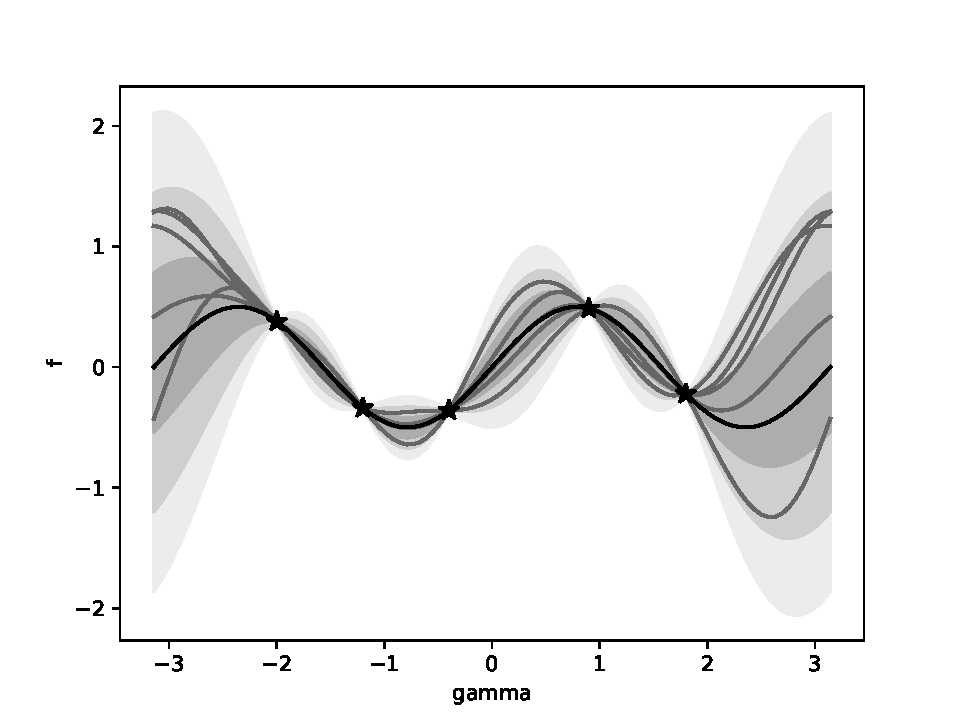
\includegraphics[width=0.43\textwidth]{img/gaussian_process.pdf}
    \caption{Output of the code. In the $x$-axis we have the angle $\gamma$, and on the $y$-axis the output of the function to an input $(\cos(\gamma_i), \sin(\gamma_i))$. The markers indicate the points that were observed and the black line the function $f$, used to generate them. The grey lines indicate possible solutions from the Gaussian Process. The shaded regions indicate the 68\%, 95\%, and 99.7\% percentiles credibility intervals (i.e.,  1, 2 and 3 standard deviations)}
    \label{fig:gp}
\end{figure}

\section{Implementing a neural network}
\label{sec:nn}

The code bellow implements the neural network described in Section~\ref{eq:nn} in PyTorch, together with the gradient descent training.

\begin{note}
    \textbf{Note:}  This code can be adapted and  used in Part 2.  The training method for Part 1 is different and does not rely on gradient descent.
\end{note}


\lstinputlisting[language=Python, caption=Implementing a neural network (available on \href{https://github.com/uu-sml/seminars-overparam-ml/blob/main/assignments/ha3-jacot/auxiliary-scripts/neural_network.py}{github.com/uu-sml/seminars-overparam-ml})]{auxiliary-scripts/neural_network.py}


\begin{figure}[H]
    \centering
    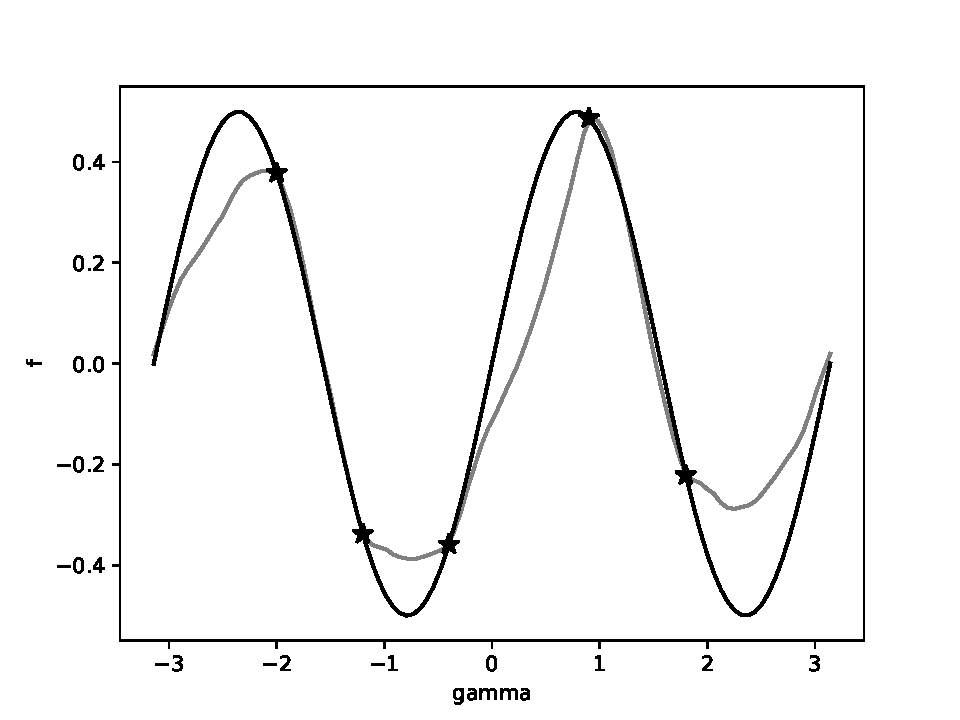
\includegraphics[width=0.43\textwidth]{img/neural_network.pdf}
    \caption{Output of the code. In the $x$-axis we have the angle $\gamma$, and on the $y$-axis the output of the function to an input $(\cos(\gamma_i), \sin(\gamma_i))$. The markers indicate the points that were observed and the black line the function $f$, used to generate them. The grey line is the neural network solution. }
    \label{fig:nn}
\end{figure}

\end{document}